\section{Matching functionals for image registration}

We regard an image $I$ as a function that maps voxels of a rectangular grid \hbox{$\mathcal{L}$}, of dimensions $n_{x} \times n_{y} \times n_{z}$ cells, to a set $G$ of
possible values called the ``dynamic range'' of $I$. The images we are interested in represent objects in physical space. This means that each point $(i,j,k)$ in the
3-dimensional grid $\mathcal{L}$ is associated to a point $(x,y,z) \in \Omega \subset \mathbf{R}^{3}$. The function that maps voxel coordinates of a grid $\mathcal{L}$ to their corresponding coordinates in physical space is an invertible affine transformation. Whenever we talk about
a grid $\mathcal{L}$ we implicitly assume that this $\mathcal{L}$ is associated to a specific grid-to-space affine transformation.
Since our images represent objects in physical space, and these objects are not tied to any specific grid, the same object may be sampled over any grid $\mathcal{L}$. Since
the grid-to-space transformation is invertible, we can, and will, unambiguously talk about images defined in physical space $\Omega \subset \mathbf{R}^{3}$.\\

\subsection{Local linear models}
Defining an adequate similarity metric between two images $I, J$ defined over $\Omega_{I}$ and $\Omega_{J}$, respectively, is arguably the most important aspect of image registration, and has been the subject of significant amount of research \citep{Sotiras2013}, if the minimum of the metric does not coincide with what we understand by optimal image correspondence, then no matter what transformation or optimization algorithm we choose, we are unlikely to correctly align the images. In the mono-modal case, a plausible model describing the input images is given by
\begin{equation}\label{eq:ssd_model}
    I(v) = J(\phi(v)) + \eta(v), \; \forall v\in\Omega_{I}
\end{equation}
where the Gaussian random variables $\eta(v) \sim N(0, \sigma^{2})$ are assumed to be independent and identically distributed. Under these assumptions, the negative log-likelihood of the observed images is proportional to the Sum of Squared Differences (SSD), given by
\begin{equation}\label{eq:ssd_functional}
    SSD(I, J; \phi) = \sum_{v \in \Omega_{I}} \left(I(v) - J(\phi(v))\right)^{2}.
\end{equation}
Thus, minimization of \eqref{eq:ssd_functional} with respect to the transformation $\phi$ corresponds to a maximum likelihood estimation of the parameters of model \eqref{eq:ssd_model} (the parameters being the transformation $\phi$). There are two main limitations of model \eqref{eq:ssd_model} in the context of brain MRI: a) it does not take into account spatial intensity inhomogeneities and b) the functional is computed \emph{point-wise}, which makes it susceptible to noise and unable to capture local image features beyond one single voxel. To overcome these limitations, \cite{Wang2014} recently proposed a local linear model that attempts to account for the bias field in brain MRI. Let $W_{v} = \left\lbrace v_{1}, v_{2}, ..., v_{n} \right\rbrace$ be a rectangular local window centered at $v\in\Omega_{I}$, containing $n$ points and denote by $\mathbf{x_{v}} = (I(v_{1}), I(v_{2}), ..., I(v_{n}))^{T}$, $\mathbf{y_{v}} = (J(\phi(v_{1})), J(\phi(v_{2})), ..., J(\phi(v_{n})))^{T}$ the input images evaluated at all points $v_{i}\in W_{v}$, $i=1, ..., n$. Please keep in mind that $\mathbf{x_{v}}$ are fixed (they never change during optimization) while $\mathbf{y_{v}}$ change as we move $\phi$ (we cannot set the value of $\mathbf{y_{v}}$ freely but their value must be adjusted by moving $\phi$). Wang's local linear model states that, when $\phi$ correctly aligns $J$ to $I$, their intensities are approximately locally linear:
\begin{equation}\label{eq:wang_model}
    \mathbf{y_{v}} = \left[\mathbf{x_{v}} \; \mathbbm{1}\right]\beta + \eta(v) \; \forall v\in\Omega_{I}
\end{equation}
where $\mathbbm{1}$ is an $n$-vector whose entries are all equal to $1$,  $\beta = (\beta_{0}, \beta_{1})^{T}$ is the vector of $2$ parameters of the local linear model and the random vectors $\eta(v)\sim N(0, \sigma^{2} \mathbbm{I}_{n})$ are assumed to be independent and identically distributed, where $\mathbbm{I}_{n}$ is the $n \times n$ identity matrix. The maximum likelihood estimator for $\beta$ can be directly computed as
\begin{equation}\label{eq:wang_model_mle_beta}
    \widehat{\beta} =
    \left[\begin{array}{cc}
        \mathbf{x_{v}}^{T}\mathbf{x_{v}} & \mathbf{x_{v}}^{T}\mathbbm{1}\\
        \mathbf{x_{v}}^{T}\mathbbm{1} & n
    \end{array}\right]^{-1}
    \left[\begin{array}{c}
        \mathbf{x_{v}}^{T}\\
        \mathbbm{1}^{T}
    \end{array}\right]\mathbf{y_{v}}.
\end{equation}
By substituting $\beta = \widehat{\beta}$ in \eqref{eq:wang_model}, and summing over all points $v\in\Omega_{I}$ the negative log-likelihood is proportional to the ``local linear reconstruction'' (LLR) matching functional, proposed by \cite{Wang2014}:
\begin{equation}\label{eq:wang_metric}
    LLR(I, J;\phi) = \sum_{v\in\Omega_{I}}|| (\mathbf{P_{v}} - \mathbbm{I})\mathbf{y_{v}}||^{2},
\end{equation}
where
\begin{equation}\label{eq:def_P_v}
    \mathbf{P_v} = [\mathbf{x_{v}} \; \mathbbm{1}]
    \left[\begin{array}{cc}
        \mathbf{x_{v}}^{T}\mathbf{x_{v}} & \mathbf{x_{v}}^{T}\mathbbm{1}\\
        \mathbf{x_{v}}^{T}\mathbbm{1} & n
    \end{array}\right]^{-1}
    \left[\begin{array}{c}
        \mathbf{x_{v}}^{T}\\
        \mathbbm{1}^{T}
    \end{array}\right].
\end{equation}
The LLR matching functional turns out to be very robust for mono-modal registration. However, in some multi-modal registration tasks, the local linear model is insufficient to describe the relationship between image modalities. To exemplify this, figure \ref{fig:llr_test} depicts an example of the residual error of local linear reconstructions between two aligned brain images (a T1 and a T2 image) from the Brainweb dataset\footnote{The Brainweb dataset was used by \cite{Wang2014} in their evaluations.}. The center image in fig. \ref{fig:llr_test} depicts the reconstruction error in false color. Although the local relationship between both images is close to linear almost everywhere, there are local regions where the intensity relationship is not close to linear regardless of what image is selected as predictor (either T1 as a function of T2 or viceversa).\\

\begin{figure}[t!]
\centering
    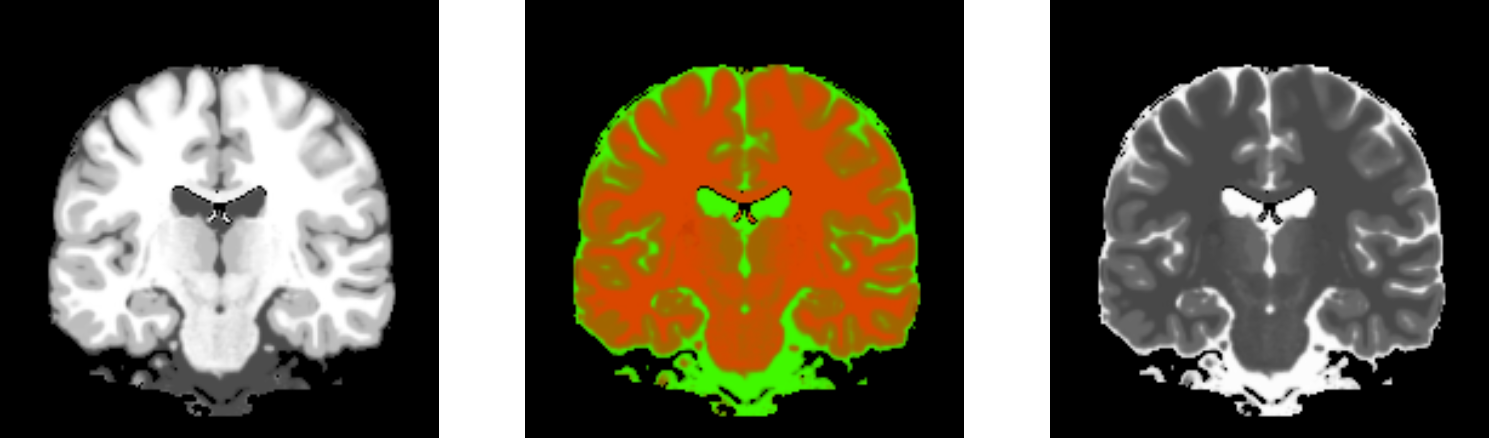
\includegraphics[width=1.0\linewidth]{./images/brainweb_t1_t2_overlay.png}\\
    \caption{Coronal slice of two realistic synthetic brain MRI images from the Brainweb dataset. The center image is an overlay of the T1 (left) image in the red channel, over the T2 (right) image in the green channel.}
\label{fig:brainweb_t1_t2}
\end{figure}

\begin{figure}[t!]
\centering
    \subfloat[]{\label{fig:T1T2_affine_fit_scatter1}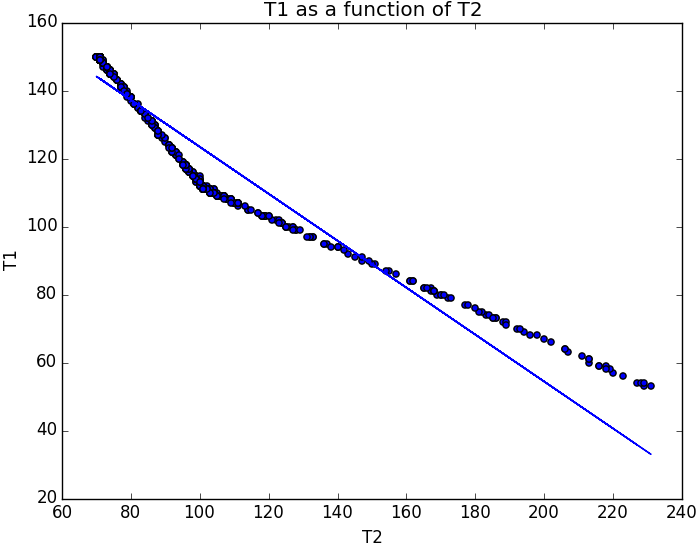
\includegraphics[width=0.2\linewidth]{./images/t1_aafo_t2_sample2.png}}
    \subfloat[]{\label{fig:T1T2_affine_fit_scatter2}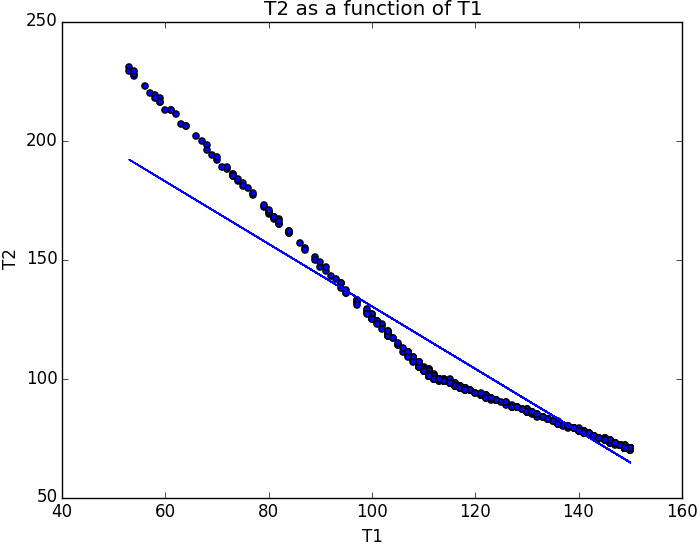
\includegraphics[width=0.2\linewidth]{./images/t2_aafo_t1_sample2.png}}
    \subfloat[]{\label{fig:T1T2_affine_fit_map}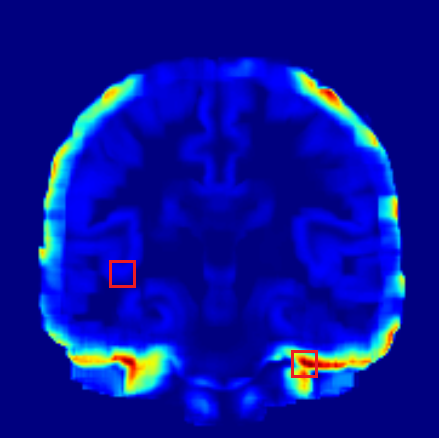
\includegraphics[width=0.2\linewidth]{./images/residuals_input.png}}
    \subfloat[]{\label{fig:T1T2_affine_fit_scatter1}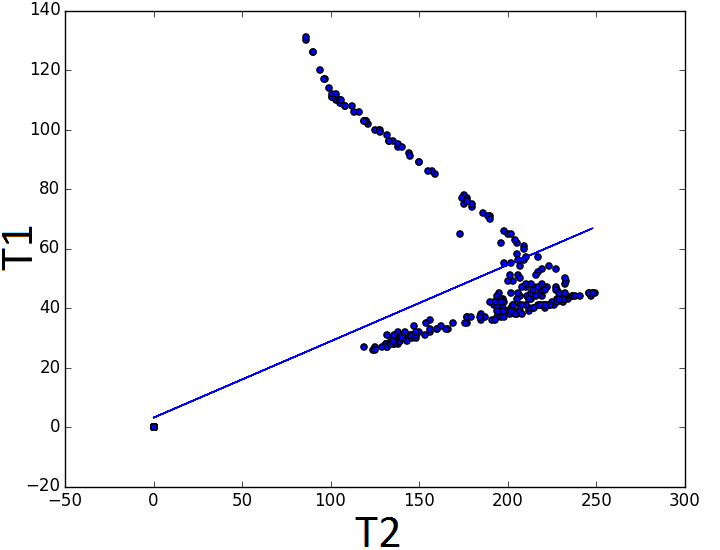
\includegraphics[width=0.2\linewidth]{./images/t1_aafo_t2_sample1.png}}
    \subfloat[]{\label{fig:T1T2_affine_fit_scatter2}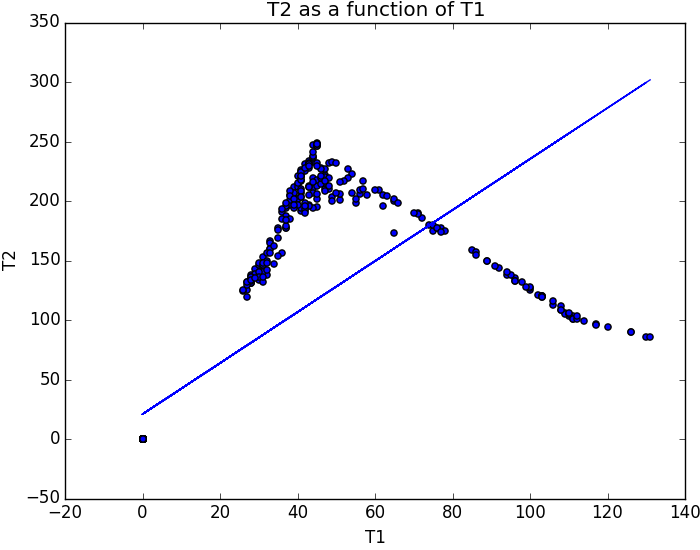
\includegraphics[width=0.2\linewidth]{./images/t2_aafo_t1_sample1.png}}\\
    \caption{Local linear reconstruction between intensities of a T1 and a T2 brain images (see fig. \ref{fig:brainweb_t1_t2}) under perfect alignment (Brainweb template). Center image (c) depicts the reconstruction error in false color (red means high reconstruction error and blue means low reconstruction error). Two local windows were selected: Left ( a)-b) ): a local window with a close-to-linear relationship between image intensities. Right (d) e) ): a local window with a non-linear relationship between image intensities. The scatter plots depict the best affine fit of T1 intensities as a function of T2 (a) and d) ), and the best fit of T2 as a function of T1 (b) and e)).}
\label{fig:llr_test}
\end{figure}

A more careful analysis of the LLR matching functional reveals that it is closely related to the popular Squared Normalized Local Cross Correlation metric, in the following sense. Note that we may assume, without loss of generality, that both vectors $\mathbf{x_{v}}, \mathbf{y_{v}}$ are \emph{centered} (i.e., their means are zero: $\frac{\mathbf{x_{v}}^{T}\mathbbm{1}}{n} = \frac{\mathbf{y_{v}}^{T}\mathbbm{1}}{n} = 0$), which may be proven as follows. Let's decompose $\mathbf{x_{v}}, \mathbf{y_{v}}$ into their centered part and their mean: $\mathbf{x_{v}} = \mathbf{x_{v}}' + \mu_{x}\mathbbm{1}$, and $\mathbf{y_{v}} = \mathbf{y_{v}}' + \mu_{y}\mathbbm{1}$, where $\mathbf{x_{v}}'$ and $\mathbf{y_{v}}'$ are centered. Then
\begin{displaymath}
    ||[\mathbf{x_{v}} \; \mathbbm{1}]\beta - \mathbf{y_{v}}||^{2} = ||[\mathbf{x_{v}}' \; \mathbbm{1}]\beta - \mathbf{y_{v}}' + \beta_{1}\mu_{x}\mathbbm{1} - \mu_{y}\mathbbm{1}||^{2} = ||[\mathbf{x_{v}}' \; \mathbbm{1}]\beta' - \mathbf{y_{v}}'||^{2}
\end{displaymath}
where $\beta' = (\beta_{1}, \beta_{0} + \beta_{1}\mu_{x} - \mu_{y})^{T}$. This $\beta'$ is the unique m.l.e. for $\beta$ in the centered case provided $\mathbf{x_{v}}$ is not a scalar multiple of $\mathbbm{1}$ (this condition makes the least squares system invertible, which makes the m.l.e. unique). This means that the LLR evaluated at non-centered vectors equals the LLR evaluated at their corresponding centered vectors. Let's consider the non-degenerate case first (the case where $\mathbf{x_{v}}$ is not a scalar multiple of $\mathbbm{1}$). In this case, as we previously showed, we can assume without loss of generality that $\mathbf{x_{v}}$ and $\mathbf{y_{v}}$ are centered. The projection matrix $\mathbf{P_{v}}$ in \eqref{eq:def_P_v} can be directly computed as
\begin{equation}\label{eq:projection_formula}
    \mathbf{P_{v}} = \frac{1}{\Delta}
    [\mathbf{x_{v}} \; \mathbbm{1}]
    \left[\begin{array}{cc}
        n & - \mathbf{x_{v}}^{T}\mathbbm{1}\\
        -\mathbf{x_{v}}^{T}\mathbbm{1} & ||\mathbf{x_{v}}||^{2}
    \end{array}\right]
    \left[\begin{array}{c}
        \mathbf{x_{v}}^{T}\\
        \mathbbm{1}^{T}
    \end{array}\right] =
    \frac{1}{n||\mathbf{x_{v}}||^{2}}
    [\mathbf{x_{v}} \; \mathbbm{1}]
    \left[\begin{array}{cc}
        n & 0\\
        0 & ||\mathbf{x_{v}}||^{2}
    \end{array}\right]
    \left[\begin{array}{c}
        \mathbf{x_{v}}^{T}\\
        \mathbbm{1}^{T}
    \end{array}\right]
\end{equation}
where $\Delta = n||\mathbf{x_{v}}||^{2} - \left(\mathbf{x_{v}}^{T}\mathbbm{1}\right)^{2} = n||\mathbf{x_{v}}||^{2} > 0$ ($||\mathbf{x_{v}}||^{2}$ cannot be zero, by hypothesis). Therefore, the entry $\mathbf{p_{i,j}}$ of $\mathbf{P_v}$ at row $i$, column $j$ is given by:
\begin{equation}
    \mathbf{p_{i,j}} = \frac{n\mathbf{x_{v}}_{i}\mathbf{x_{v}}_{j} + ||\mathbf{x_v}||^{2}}{n||\mathbf{x_{v}}||^{2}}.
\end{equation}
Each term of the LLR metric (corresponding to the local window centered at voxel $v$) can be writen as:
\begin{displaymath}
    ||(\mathbf{P_{v}} - \mathbbm{I})\mathbf{y_{v}}||^{2} = \sum_{i=1}^{n} \left(\sum_{j=1}^{n} \mathbf{p_{i,j}} \mathbf{y_{v}}_{j} - \mathbf{y_{v}}_{i}\right)^{2} =
    \sum_{i=1}^{n}\left(\frac{\mathbf{x_{v}}^{T}\mathbf{y_{v}}}{||\mathbf{x_{v}}||^{2}} \mathbf{x_{v}}_{i} - \mathbf{y_{v}}_{i}\right)^{2} = ||\mathbf{y_{v}}||^{2} - \frac{(\mathbf{x_{v}}^{T}\mathbf{y_{v}})^{2}}{||\mathbf{x_{v}}||^{2}} =
\end{displaymath}
\begin{equation}\label{eq:llr_cc_relationship}
    = ||\mathbf{y_{v}}||^{2}\left(1 - \frac{(\mathbf{x_{v}}^{T}\mathbf{y_{v}})^{2}}{||\mathbf{x_{v}}||^{2}||\mathbf{y_{v}}||^{2}}\right).
\end{equation}
Therefore, the LLR functional may be regarded as a modified Cross Correlation with a bias towards making $||\mathbf{y_{v}}||$ small (note that the CC metric operates on centered local vectors too). This bias may be removed from model \eqref{eq:wang_model} by normalizing $\mathbf{y_{v}}$:\\
\begin{equation}\label{eq:normalized_ll_model}
    \frac{\mathbf{y_{v}}}{||\mathbf{y_{v}}||} = \left[\mathbf{x_{v}} \; \mathbbm{1}\right]\beta + \eta(v) \; \forall v\in\Omega_{I},
\end{equation}
and we can see that maximization of likelihood under model \eqref{eq:normalized_ll_model} is now equivalent to maximization of the local cross correlation metric.\\

\subsection{Global non-linear transfer}
The matching functional we propose in this work is based on the empirical observation that, the non-linear relationship between both image modalities at local windows (fig. \ref{fig:llr_test}) may be made closer to linear by applying a global, non-linear, transfer function $F: G \rightarrow \mathbbm{R}$ that maps intensities from one modality to the other (fig. \ref{fig:ecc_test_good}). More precisely, our model may be written as
\begin{equation}\label{eq:ecc_model}
    \frac{\mathbf{y_{v}}}{||\mathbf{y_{v}}||} = \left[F\left[\mathbf{x_{v}}\right] \; \mathbbm{1}\right]\beta + \eta(v) \; \forall v\in\Omega_{I},
\end{equation}
where we have denoted $F[\mathbf{x_{v}}]$ the vector that results from applying function $F$ to each element of vector $\mathbf{x_{v}}$. By following the exact same steps as before, we can compute the optimal regression parameters $\widehat{\beta}$ and obtain the negative log-likelihood of our data under model \eqref{eq:ecc_model} (by replacing $\mathbf{x_{v}}$ with $F[\mathbf{x_{v}}]$ and $\mathbf{y_{v}}$ with $\frac{\mathbf{y_{v}}}{||\mathbf{y_{v}}||}$ in eq. \eqref{eq:llr_cc_relationship}):
\begin{equation}\label{eq:ecc_neg_likelihood}
    U(I, J;\phi) = \sum_{v\in\Omega_{I}}\left(1-\frac{\left(F\left[\mathbf{x_{v}}\right]^{T} \mathbf{y_{v}}\right)^{2}}{||F\left[\mathbf{x_{v}}\right]||^{2}||\mathbf{y_{v}}||^{2}}\right).
\end{equation}
The minimum of \eqref{eq:ecc_neg_likelihood} can be obtain by maximizing our proposed matching functional, which we call \emph{Expected Cross Correlation} (the reason of this name will be clear soon):
\begin{equation}\label{eq:ecc_functional}
    ECC(I, J;\phi) = \sum_{v\in\Omega_{I}}\frac{\left(F\left[\mathbf{x_{v}}\right]^{T} \mathbf{y_{v}}\right)^{2}}{||F\left[\mathbf{x_{v}}\right]||^{2}||\mathbf{y_{v}}||^{2}}.
\end{equation}
Now we will proceed to compute an optimal non-linear transfer function $F$. We can see from model \eqref{eq:ecc_model}, that the optimal function $F$ is not unique: if $F^{*}$ is optimal, then any affine transform of $F^{*}$, say $\widehat{F} = \alpha_{0} F^{*} + \alpha_{1}\mathbbm{1}$ is optimal too, because:
\begin{displaymath}
    \left[\widehat{F}\left[\mathbf{x_{v}}\right] \; \mathbbm{1}\right]\beta =
    \left[\left(\alpha_{0}F^{*}\left[\mathbf{x_{v}}\right]+\alpha_{1}\mathbbm{1}\right) \; \mathbbm{1}\right]\beta =
    \left[F^{*}\left[\mathbf{x_{v}}\right] \; \mathbbm{1}\right]\beta',
\end{displaymath}
where $\beta' = (\alpha_{0}\beta_{0}, \alpha_{1}\beta_{0} + \beta_{1})^{T}$. Therefore, what we want to find is the optimal $F$ modulo an affine transform. Let's denote by $m$ the number of different intensity values in the fixed image $I$ (a typical choice is $m=256$). We aim to assign a value $\mathbf{f}_{\ell}$ to each intensity $\ell$ of the fixed image, $0\leq \ell < m$, and define the transfer function $F$ as $F(\mathbf{x_{v}}_{i}) = \mathbf{f}_{\ell}$, where $\ell = \mathbf{x_{v}}_{i}$. The transfer function $F$ may then be represented as a vector $\mathbf{f}$ of dimension $m$. Let $\mathbf{k_{v}}_{\ell}$, and $\mathbf{a_{v}}_{\ell}$ be number of elements of $\mathbf{x_{v}}$ equal to $\ell$, and the sum of elements of $\mathbf{y_{v}}$ whose corresponding elements in $\mathbf{x_{v}}$ equal $\ell$, respectively. More precisely:
\begin{displaymath}
    \mathbf{k_{v}}_{\ell} = |\left\lbrace i : \mathbf{x_{v}}_{i}=\ell \right\rbrace|
\end{displaymath}
\begin{displaymath}
    \mathbf{a_{v}}_{\ell} = \sum_{i:\mathbf{x_{v}}_{i}=\ell} \mathbf{y_{v}}_{i}
\end{displaymath}
then, the dot product in equation \eqref{eq:ecc_neg_likelihood} may be written in term of $\mathbf{f}$ as follows:
\begin{displaymath}
    F\left[\mathbf{x_{v}}\right]^{T} \mathbf{y_{v}} = \sum_{\ell=1}^{m} \sum_{i:\mathbf{x_{v}}_{i}=\ell} F(\mathbf{x_{v}}_{i})\mathbf{y_{v}}_{i}
    =\sum_{\ell=1}^{m} \mathbf{f_{\ell}}\mathbf{a_{v}}_{\ell} = \mathbf{f}^{T}\mathbf{a_{v}}
\end{displaymath}
and the squared norm $||F[\mathbf{x_{v}}]||^{2}$ as:
\begin{displaymath}
    ||F\left[\mathbf{x_{v}}\right]||^{2} = \sum_{\ell=1}^{m} \sum_{i:\mathbf{x_{v}}_{i}=\ell} F(\mathbf{x_{v}}_{i})^{2}
    = \sum_{\ell=1}^{m} \mathbf{f_{\ell}}^{2} \mathbf{k_{v}}_{\ell} = \mathbf{f}^{T} \mathbf{D_{v}} \mathbf{f}
\end{displaymath}
where $\mathbf{D_{v}} = $ diag($\mathbf{k_{v}}$). Equation \eqref{eq:ecc_functional} can be written as:
\begin{equation}\label{eq:ecc_neg_likelihood_vector_form}
    ECC(I, J;\phi) = \sum_{v\in\Omega_{I}}\frac{\mathbf{f}^{T}\mathbf{a_{v}}\mathbf{a_{v}}^{T}\mathbf{f}}
    {\mathbf{f}^{T} \mathbf{D_{v}} \mathbf{f}||\mathbf{y_{v}}||^{2}}.
\end{equation}
The problem of maximizing the sum of quotients of quadratic forms, like eq. \eqref{eq:ecc_neg_likelihood_vector_form} doesn't have, in general, a close form solution, and it is necessary to resort to iterative algorithms (see for example \cite{Kiers1995} for a thorough review of this problem). The sole evaluation of the functional may be very time consuming because in order to apply fast strategies like partial sums (used for example by \cite{Avants2008} to evaluate the CC metric and its gradient) we need to store the partial results for each intensity value $0 \leq \ell < m$, which would require a very large amount of memory. Therefore, we will compute an approximation based on the following assumptions.\\

1. The set of intensities of each each vector $\mathbf{x_{v}}$ are approximately a random sample from intensities of image $I$. Then, the number $\mathbf{k_{v}}_{\ell}$ of vector elements $i$ where $\mathbf{x_{v}}_{i} = \ell$, may be approximated by its expected value $n\mathbf{p}_{\ell}$, where the probability $\mathbf{p}_{\ell}$ of a voxel having intensity $\ell$ may be estimated by the empirical probability:
\begin{equation}
    \mathbf{k_{v}}_{\ell} \approx \mathbbm{E}[\mathbf{k_{v}}_{\ell}] \approx n\frac{|\left\lbrace v\in\Omega_{I} : I(v) = \ell\right\rbrace|}{|\Omega_{I}|} := n\mathbf{p}_{\ell},
\end{equation}
and from this approximation it follows that $\frac{1}{n}\mathbf{D_{v}} \approx $diag$(\mathbf{p}) := \mathbf{P}$.\\

2. The average $\frac{\mathbf{a_{v}}_{\ell}}{\mathbf{k_{v}}_{\ell}}$ of all elements of vector $\mathbf{y_{v}}$ whose corresponding entries in $\mathbf{x_{v}}$ are equal to $\ell$ may be approximated by the average computed over the full image $J$, where intensities in $I$ are equal to $\ell$:
\begin{equation}
    \frac{\mathbf{a_{v}}_{\ell}}{\mathbf{k_{v}}_{\ell}} =  \frac{1}{\mathbf{k_{v}}_{\ell}}\sum_{i:\mathbf{x_{v}}_{i}=\ell} \mathbf{y_{v}}_{i} \approx \frac{1}{|G_{\ell}|}\sum_{v\in G_{\ell}} J(\phi(v))
    :=\bar{\mathbf{f}}_{\ell},
\end{equation}
where $G_{\ell} = \left\lbrace v\in \Omega_{I}: I(v) = \ell\right\rbrace$. From these conditions, it follows that $\mathbf{a_{v}}_{\ell} \approx n \mathbf{P} \mathbf{\bar{f}}$.

3. The norm $||\mathbf{y_{v}}||$ is approximately equal to $||F[\mathbf{x_{v}}]||$.
\begin{equation}
    ||\mathbf{y_{v}}|| \approx ||F[\mathbf{x_{v}}]|| \; \forall v\in\Omega_{I}
\end{equation}

Notice that, if the local windows $W_{v}, v\in\Omega_{I}$ are sufficiently large, then these two conditions are satisfied (to convince ourselves, it suffices to consider the extreme case of one single ``local'' window of size equal to the full image). The question is how small can we make the local windows so that these conditions are reasonably satisfied. Please note that we do not need all the conditions to be satisfied everywhere, in practice we only need that the optimal $\mathbf{f}$ obtained under the given assumptions is reasonably close to the optimal $\mathbf{f}$ obtained without making the assumptions. From our experiments, as we will show below, we have found that rectangular local windows of radius $4$ voxels work remarkably well in practice.\\

Under the conditions stated above, eq. \eqref{eq:ecc_neg_likelihood_vector_form} can be approximated as
\begin{equation}
    \sum_{v\in\Omega_{I}}\frac{\mathbf{f}^{T}\mathbf{a_{v}}\mathbf{a_{v}}^{T}\mathbf{f}}
    {\mathbf{f}^{T} \mathbf{D_{v}} \mathbf{f}||\mathbf{y_{v}}||^{2}} \approx 
    \frac{n^{2}|\Omega_{I}|}{n^{2}}
    \frac{\mathbf{f}^{T}\mathbf{P}\mathbf{\bar{f}}\mathbf{\bar{f}}^{T}\mathbf{P}^{T}\mathbf{f}}{\left(\mathbf{f}^{T} \mathbf{P} \mathbf{f}\right)^{2}}.
\end{equation}

By making the change of variables $\mathbf{h} = \mathbf{P}^{\frac{1}{2}}\mathbf{f}$, we obtain:
\begin{equation}\label{eq:ecc_neg_likelihood_vector_form_simplified}
    |\Omega_{I}|
    \frac{\mathbf{f}^{T}\mathbf{P}\mathbf{\bar{f}}\mathbf{\bar{f}}^{T}\mathbf{P}^{T}\mathbf{f}}{\left(\mathbf{f}^{T} \mathbf{P} \mathbf{f}\right)^{2}} \approx 
    |\Omega_{I}| \frac{\mathbf{h}^{T}\mathbf{P}^{\frac{1}{2}}\mathbf{\bar{f}}\mathbf{\bar{f}}^{T}\mathbf{P}^{\frac{1}{2}}\mathbf{h}} {\left(\mathbf{h}^{T}\mathbf{h}\right)^{2}} =
    |\Omega_{I}| \frac{\mathbf{h}^{T}\mathbf{\bar{h}}\mathbf{\bar{h}}^{T}\mathbf{h}} {\left(\mathbf{h}^{T}\mathbf{h}\right)^{2}}
\end{equation}
where $\mathbf{\bar{h}} := \mathbf{P}^{\frac{1}{2}}\mathbf{\bar{f}}$. Since we are interested in finding the optimal $\mathbf{f}$ modulo affine transforms, we may without loss of generality maximize eq. \eqref{eq:ecc_neg_likelihood_vector_form_simplified} subject to $||\mathbf{h}|| = ||\mathbf{\bar{h}}||$, which yields solution $\mathbf{h} = \mathbf{\bar{h}}$, and by definition, $\mathbf{f} = \mathbf{P}^{-\frac{1}{2}}\mathbf{h} = \mathbf{\bar{f}}$.\\

The effect of introducing this global non-linear transfer into the local linear model is illustrated in fig. \ref{fig:ecc_test_good}. This example is the same as fig. \ref{fig:llr_test}, the fixed image $I$ is the T1, the moving image $J$ is the T2, but instead of fitting the local linear models between $I$ and $J$ directly as in \cite{Wang2014}, we used $F[I]$ and $J$, where $F$ is defined by the approximated optimal vector $\mathbf{\bar{f}}$, as explained above. It can be observed that the non-linear local relationship was made significantly closer to linear by the use of the global transfer function.\\

\begin{figure}[t!]
\centering
    \subfloat[]{\label{fig:FT1T2_affine_fit_scatter1}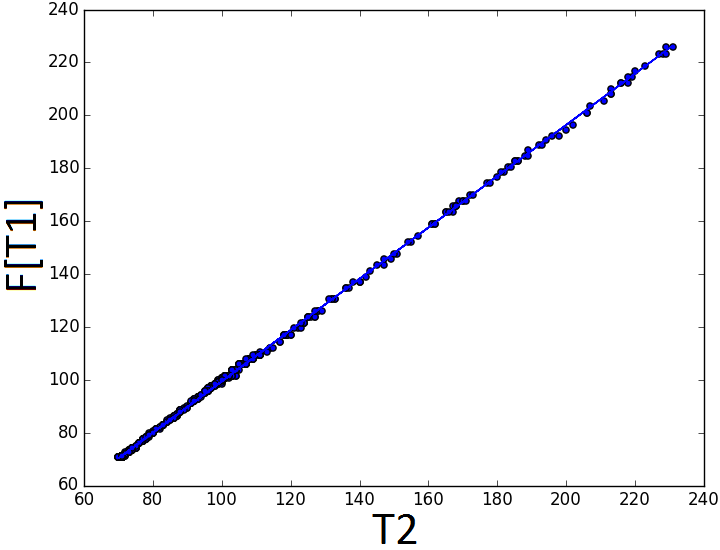
\includegraphics[width=0.2\linewidth]{./images/Ft1_aafo_t2_sample2.png}}
    \subfloat[]{\label{fig:FT1T2_affine_fit_scatter2}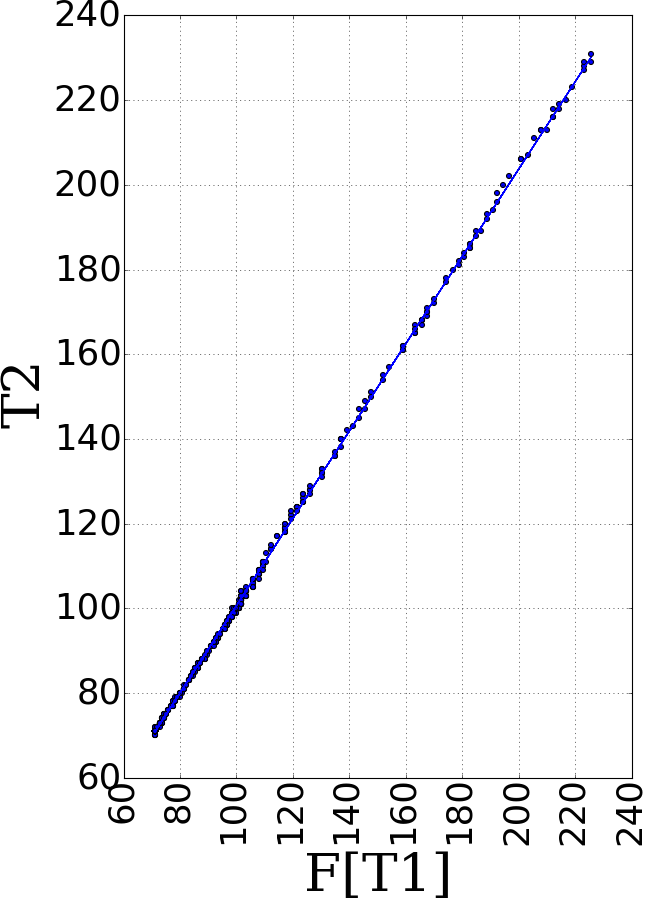
\includegraphics[width=0.2\linewidth]{./images/t2_aafo_Ft1_sample2.png}}
    \subfloat[]{\label{fig:FT1T2_affine_fit_map}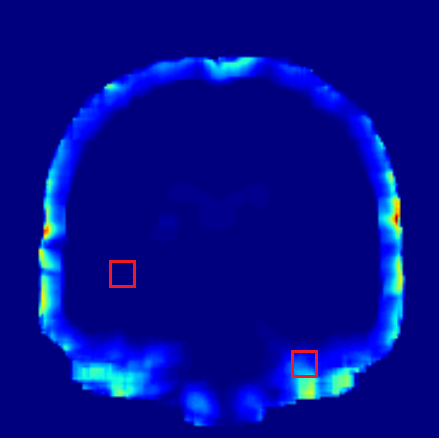
\includegraphics[width=0.2\linewidth]{./images/residuals_t2.png}}
    \subfloat[]{\label{fig:FT1T2_affine_fit_scatter1}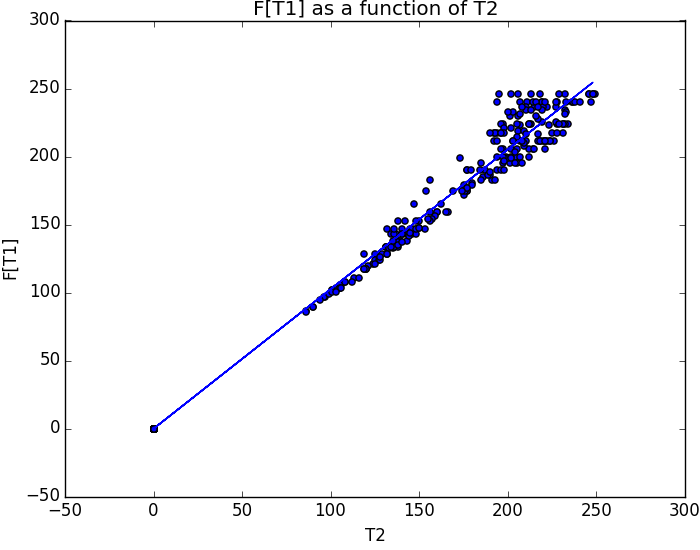
\includegraphics[width=0.2\linewidth]{./images/Ft1_aafo_t2_sample1.png}}
    \subfloat[]{\label{fig:FT1T2_affine_fit_scatter2}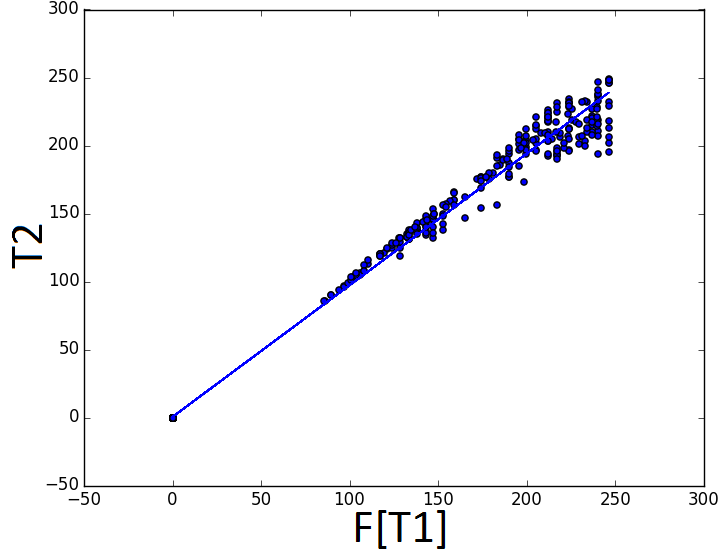
\includegraphics[width=0.2\linewidth]{./images/t2_aafo_Ft1_sample1.png}}\\
    \caption{Local linear reconstruction between T2 intensities and F[T1], where F is the global transfer function used in the Correlation Ratio metric (the average T2 intensity computed over iso-sets of the T1). Center image (c) depicts the reconstruction error in false color (red means high, and blue means low). The selected windows are the same as in figure \ref{fig:llr_test}. The scatter plots depict the best affine fit of F[T1] intensities as a function of T2 (a) and d) ), and the best fit of T2 as a function of F[T1] (b) and e)).}
\label{fig:ecc_test_good}
\end{figure}

A limitation of matching functionals that are based on the assumption of some kind of functional dependency between image intensities is that one of the image modalities must be chosen \emph{a priori} as the target modality (either map intensities from modality A to modality B or viceversa). This is an important decision and what choice is the best may not be obvious in general. Figure \ref{fig:ecc_test_bad} shows the same example as fig. \ref{fig:ecc_test_good}, but instead of mapping intensities from T1 to T2, we map intensities from T2 to T1. Although the transfer function from T2 to T1 helped, the relationship is still non-linear. Our matching functional considers both transfer functions, eliminating the need for a target modality to be chosen beforehand.\\

\begin{figure}[t!]
\centering
    \subfloat[]{\label{fig:T1FT2_affine_fit_scatter1}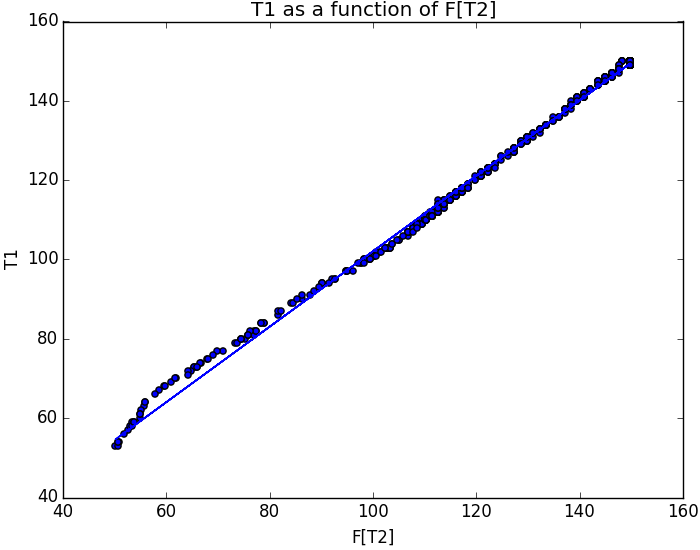
\includegraphics[width=0.2\linewidth]{./images/t1_aafo_Ft2_sample2.png}}
    \subfloat[]{\label{fig:T1FT2_affine_fit_scatter2}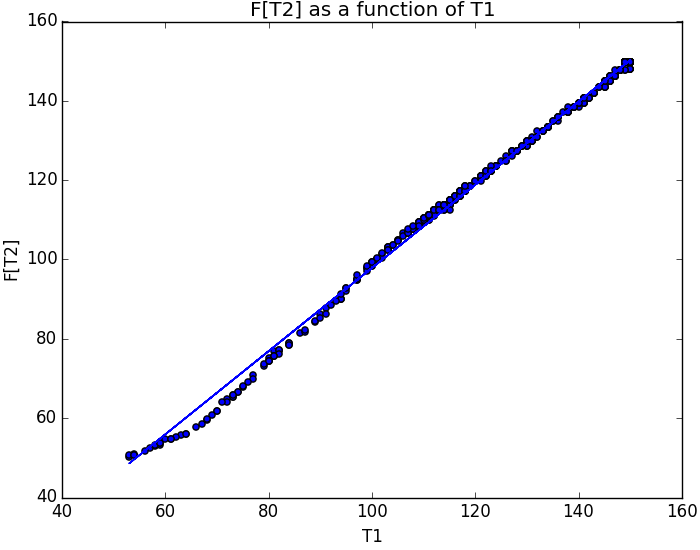
\includegraphics[width=0.2\linewidth]{./images/Ft2_aafo_t1_sample2.png}}
    \subfloat[]{\label{fig:T1FT2_affine_fit_map}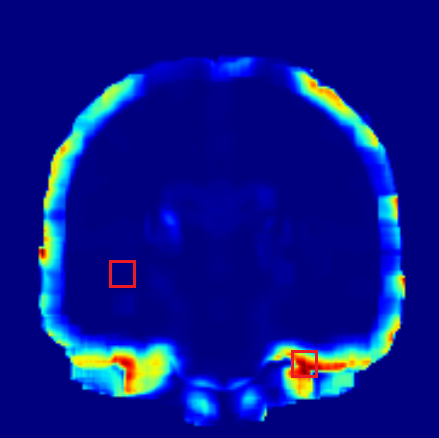
\includegraphics[width=0.2\linewidth]{./images/residuals_t1.png}}
    \subfloat[]{\label{fig:T1FT2_affine_fit_scatter1}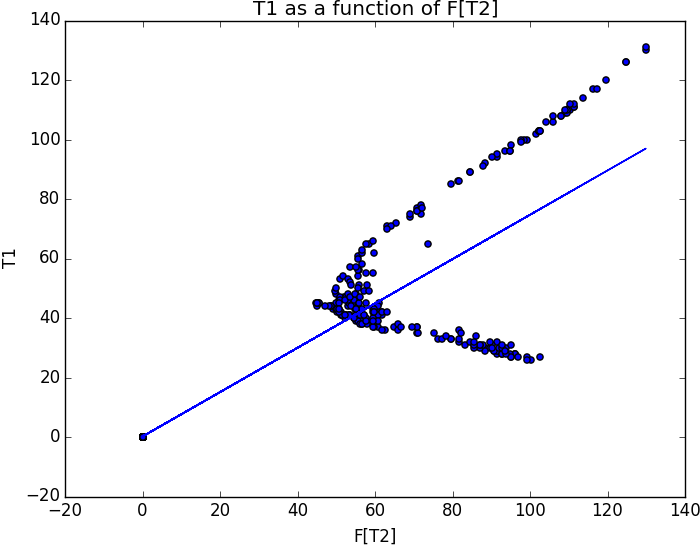
\includegraphics[width=0.2\linewidth]{./images/t1_aafo_Ft2_sample1.png}}
    \subfloat[]{\label{fig:T1FT2_affine_fit_scatter2}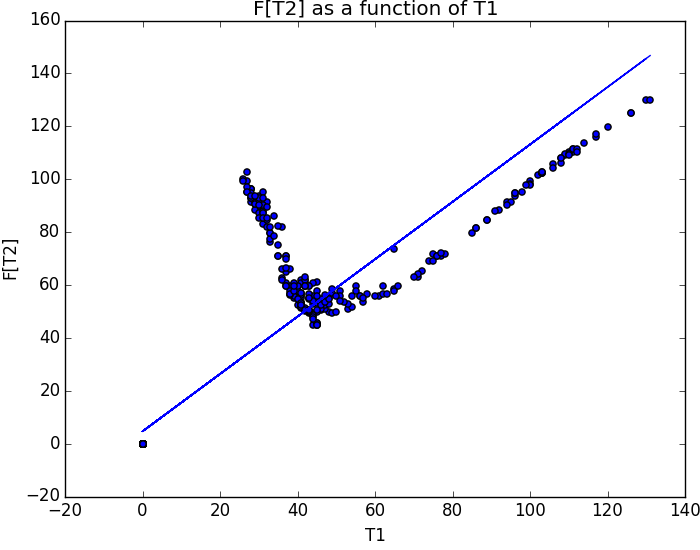
\includegraphics[width=0.2\linewidth]{./images/Ft2_aafo_t1_sample1.png}}\\
    \caption{.}
\label{fig:ecc_test_bad}
\end{figure}








Recently, \cite{Arce-santana2014} modeled the transfer function between the image modalities as
\begin{equation}\label{eq:arce_model}
    F[I(x)] = J(\phi(x)) + \eta(x), x\in \mathcal{L}
\end{equation}
where $F$ is the (unknown) transfer function between image modalities and $\eta(x), x\in \mathcal{L}$ are independent random variables with Gaussian distribution. Since the grid $\mathcal{L}$ is discrete, image $F[I(x)], x\in \mathcal{L}$ may be modeled as a discrete set of hidden random variables $Y(x) = F[I(x)]$ whose distribution parameters
can be estimated using the Expectation Maximization (EM) algorithm \citep{Dempster1977}. In their work, \cite{Arce-santana2014} used a discretized elastic
deformation model to test the behavior of their metric, which leads to the following energy minimization problem

\begin{equation}\label{eq:arce_elastic}
    \mathbf{u}^{*} = \arg \min_{\mathbf{u}} \sum_{x \in \mathcal{L}} \frac{1}{2 \sigma(x)^{2}} ( \bar{I}(x) - J(x + \mathbf{u}(x)))^{2} + \lambda \sum_{<x, y>} ||\mathbf{u}(x) - \mathbf{u}(y)||^{2},
\end{equation}
where $\bar{I}(x), \sigma(x), x\in \mathcal{L}$ are the estimated parameters (mean and standard deviation) of the hidden variable $F[I(x)]$ given the
observed intensity $I(x)$ and $<x, y>$ denote neighboring pixels in $\mathcal{L}$. Even though the authors only evaluated their metric for 2D image registration and used
the elastic model, this formulation can be extended, as we will show in the next section, to develop an efficient and accurate symmetric diffeomorphic non-linear registration algorithm for 3D multi-modal images by taking advantage of the ideas of Avants' \textit{Greedy SyN} \citep{Avants2008}, Vercauteren's \textit{Diffeomorphic Demons} \citep{Vercauteren2009} and Arce's \textit{EM transfer function} model \citep{Arce-santana2014}.

\subsection{Symmetric diffeomorphic registration}

The goal of image registration is to compute a transformation $\phi: \Omega \rightarrow \Omega$ that brings a moving image $J:\Omega \rightarrow G$ into correspondence
with a fixed image $I:\Omega \rightarrow G$. The transformation $\phi$ is chosen from a set $\Phi$ of feasible solutions having properties that are desirable depending on the
application, such as smoothness and invertibility. Correspondence between $I$ and $J$ is defined to be reached when a dissimilarity metric between them is minimized.\\

In non-linear image registration, the transformation $\phi$ is usually represented by a deformation field $\mathbf{u(\cdot)}$ that assigns a displacement vector
to each point $x$ such that $\phi(x) = x + \mathbf{u}(x)$. The classical elastic model is one of the earliest formulation for non-linear image registration \citep{Bajcsy1982, Gee1999},
and may be written as

\begin{equation}\label{eq:elastic}
    \mathbf{u}^{*} = \arg \min_{\mathbf{u}} \int_{\Omega} ||L \mathbf{u}(x)||^{2}dV + \Pi(I, J \circ \phi),
\end{equation}
where $L$ is a differential operator used to promote smoothness on $\mathbf{u}$ and $\Pi$ is the dissimilarity metric driving the registration. A limitation of this model, especially important for medical image registration is that the solution, although being smooth, is not guaranteed to be invertible, and the topology of the moving image is not guaranteed to be preserved after transforming it under $\phi$.\\

To overcome the limitations of the elastic model, the large deformation proposed by \cite{Christensen2001} and further developed by \cite{Science2005} formulates the problem in terms of a trajectory of transformations \hbox{$\phi:\Omega_{I} \times [0, 1] \rightarrow \Omega_{J}$} that satisfies $\frac{d \phi(x, t)}{dt} = v(\phi(x, t), t)$ and $\phi(x, 0) = x$, where $v(\cdot, \cdot)$ is
the velocity field associated to the curve $\phi$. Beg's Large Deformation Diffeomorphic Metric Mapping (LDDMM) \citep{Science2005} formulation of the registration problem is given by:
\begin{equation}\label{eq:LDDMM}
    v^{*} = \arg \min_{v:\dot{\phi} = v_{t}(\phi)} \int_{0}^{1} ||L v_{t}||^{2} dt + \Pi(I, J \circ \phi(\cdot, 1)),
\end{equation}
where $\dot{\phi} = \frac{d\phi}{dt}$, $v_{t} = v(\cdot, t), t\in [0, 1]$. The final diffeomorphisms can be obtained by integrating over time
\begin{equation}\label{eq:velocity_integral}
    \phi(x, 1) = \phi(x, 0) + \int_{0}^{1}v(\phi(x, t), t) dt.
\end{equation}

\cite{Dupuis1998} showed that by enforcing sufficient smoothness in $v$, through the differential operator $L$, it can be guaranteed that $\phi(\cdot, t), t \in [0, 1]$ are diffeomorphisms. This and other formulations also based on diffeomorphic flows ensure that images are smoothly transformed and their topology preserved: an important property for many medical applications. \cite{Avants2008, Avants2011} modified the standard LDDMM formulation to enforce symmetry in the sense that the registration result is the same regardless of which image we designate as $I$ and $J$. This property, although natural and desirable, is not ensured in standard computational methods solving the LDDMM problem. By splitting the trajectory $\phi$ into two trajectories with opposite direction $\phi_{1}(x, t) = \phi_{2}(y, 1-t)$, where $y = \phi(x, 1)$, with corresponding velocity fields $v_{1}, v_{2}$, the Symmetric formulation for Diffemorphic Image Registration \citep{Avants2008, Avants2011} can be written as:

\begin{equation}\label{eq:syn_energy}
    \begin{array}{lll}
        v_{1}^{*}, v_{2}^{*} &=& \mathlarger{\arg \min \int_{t=0}^{0.5} ||L v_{1}(x, t)||^{2} + ||L v_{2}(x, t)||^{2} dt}\\
        &+& \mathlarger{ \Pi(I \circ \phi_{1}(\cdot, 0.5), J(\phi_{2}(\cdot, 0.5)))}
    \end{array}
\end{equation}
subject to
\begin{equation}\label{eq:syn_energy_constraints}
    \begin{array}{l}
        \frac{d\phi_{i}(x, t)}{dt} = v_{i}(\phi(x,t),t)\\
        \phi_{i}(\cdot, 0) = \mathbf{I},\, \phi_{i}^{-1}(\phi_{i}) = \mathbf{I},\, \phi_{i}(\phi_{i}^{-1}) = \mathbf{I},\, i=1,2,
    \end{array}
\end{equation}
where $\mathbf{I}$ denotes the identity transformation. \cite{Avants2006} proposed a numerical algorithm, called \textit{Geodesic SyN} for solving \eqref{eq:syn_energy}, which deforms both images towards the midpoint of the trajectory. The main drawback of directly solving eq. \eqref{eq:syn_energy} is its computational cost, since it requires space and time discretization and it is necessary to integrate the velocity fields in eq. \eqref{eq:velocity_integral} to obtain the trajectories at each iteration. A more efficient optimization algorithm to approximately solve eq. \eqref{eq:syn_energy}, also proposed by \cite{Avants2008, Avants2011}, consists in computing the gradient of the metric only at the midpoint of the trajectory (as opposed to evaluating it for all time):
\begin{equation}\label{eq:grad_metric}
    \nabla_{\phi_{i}} \Pi(\tilde{I}, \tilde{J}) = \frac{\partial}{\partial \phi_{i}} \Pi \left( \tilde{I}, \tilde{J}\right),
\end{equation}
where $\tilde{I} = I \circ \phi_{1}^{-1}(\cdot, 0.5)$, $\tilde{J} = J \circ \phi_{2}^{-1}(\cdot, 0.5)$. The midpoint diffeomorphisms are then updated by composition with the gradient after smoothing with a Gaussian kernel $K_{\sigma}$ (as opposed to integrating along the full geodesic)

\begin{equation}\label{eq:gsyn_update}
    \phi_{i}(\cdot, 0.5) = \phi_{i}(\cdot, 0.5) - \left( \epsilon K_{\sigma} \ast \nabla_{\phi_{i}} \Pi(\tilde{I}, \tilde{J}) \right) \circ \phi_{i}(\cdot, 0.5),
\end{equation}
where $\ast$ denotes the convolution operator and $\epsilon$ is a small factor controlling the step size in the optimization process. Finally, the updated midpoint transformations (which, after composition with the gradient, are not ensured to be diffeomorphisms) are forced to be invertible by using an explicit vector field inversion algorithm \citep{Chen2008}. This algorithm, called \textit{Greedy SyN} (see Appendix \ref{ap:Algorithms}, alg. \ref{alg:Greedy_SyN}) has been adopted by the neuroimaging community as the \textit{de facto} state-of-the-art brain MRI registration algorithm due to its reliability and efficiency. It was the method used for evaluating ANTS \citep{Avants2011} in the large comparative studies developed by \cite{Klein2009, Klein2010} in which \textit{Greedy SyN} consistently ranked first.


